\documentclass[11pt]{article}
\usepackage[T1]{fontenc}
\usepackage[utf8]{inputenc}
\usepackage{lmodern}
\usepackage{microtype}
\usepackage[margin=1in]{geometry}
\usepackage{setspace}
\usepackage{amsmath,amssymb,amsthm}
\usepackage{mathtools}
\usepackage{bm}
\usepackage{graphicx}
\usepackage{booktabs}
\usepackage{tabularx}
\usepackage{array}
\usepackage{enumitem}
\usepackage{xcolor}
\usepackage{caption}
\usepackage{subcaption}
\usepackage{tikz}
\usetikzlibrary{arrows.meta,positioning,calc,decorations.pathreplacing}
\usepackage[authoryear,round]{natbib}
\usepackage{xurl}
\usepackage{xr}
\usepackage[hidelinks]{hyperref}
\usepackage{cleveref}

\theoremstyle{plain}
\newtheorem{proposition}{Proposition}
\newtheorem{lemma}{Lemma}
\newtheorem{corollary}{Corollary}
\theoremstyle{definition}
\newtheorem{assumption}{Assumption}
\newtheorem{definition}{Definition}
\theoremstyle{remark}
\newtheorem{remark}{Remark}

\crefname{proposition}{Proposition}{Propositions}
\crefname{lemma}{Lemma}{Lemmas}
\crefname{corollary}{Corollary}{Corollaries}
\crefname{assumption}{Assumption}{Assumptions}
\crefname{remark}{Remark}{Remarks}
\crefname{definition}{Definition}{Definitions}
\crefname{section}{Section}{Sections}
\crefname{subsection}{Section}{Sections}
\crefname{appendix}{Appendix}{Appendices}
\crefname{subappendix}{Appendix}{Appendices}
\crefname{table}{Table}{Tables}
\crefname{figure}{Figure}{Figures}
\crefname{equation}{equation}{equations}
\creflabelformat{equation}{(#2#1#3)}


\newcommand{\pos}[1]{\left[#1\right]^{+}}
\setlist{itemsep=2pt,topsep=4pt}

\externaldocument{supplement}
\onehalfspacing

% Set to true for a version without author information (double-blind review).
\newif\ifanonymous
\anonymousfalse

\title{Owning the Chokepoint: ASML, Alliance Dependence, and the Limits of Europe's Leverage over Washington}
\ifanonymous
\author{}
\else
\author{Matt DiGiuseppe\thanks{Working draft, \today. Almost all of this paper was written by Claude, an AI system made by Anthropic, working in Claude Code. Claude wrote the model, the proofs, the numerical checks, the literature and fact review, the text, the tables and the figures. Matt DiGiuseppe's contribution was the research question, the instructions and the reading material (including the \emph{Europe 2031} scenario). Results were spot-checked numerically by brute-force computation, which is not formal verification. An online supplement states the extensions and gives every proof and the numerical checks; references to sections, results and tables numbered with an S are to the supplement.} \and Claude (Anthropic)}
\fi
\date{\today}

\begin{document}
\maketitle

\begin{abstract}
\noindent Since 2019 the Netherlands, home of ASML, sole maker of extreme ultraviolet lithography machines, has aligned its export controls with US demands for little in return. So has Japan since 2023. Yet both resist limits on servicing in China. In our model a security-dependent chokepoint holder (Europe) bargains with its patron while a rival bids for it. The holder's exit premium, the rival's credible offer net of the credible costs of exit, is a floor on what it obtains; unless the holder makes proposals in talks that can rupture for long, or can hurt the patron while they bargain, its leverage is the positive part of that premium. Whatever bargaining sets the holder's price, its surplus over exit bounds what the patron's conditional threats can extract. Demands compete for that budget only where the patron enforces them through the alliance itself. Refusals need a patron unsure of what a demand costs, and near a zero premium its threats can prevent fewer of them. Any surplus that a transfer of control would remove gives the patron a preventive motive to demand control. US jurisdiction over ASML's inputs and staff can keep Europe's premium negative without any security term. Beyond that, its sign turns on China's credible promises and on any credible US threat to withhold frontier AI, which on our orders of magnitude outweighs the conditional part of the US guarantee.

\end{abstract}

\newpage
\section{Introduction}\label{sec:intro}

In \emph{Europe 2031}, a scenario published in June 2026 by eight authors writing in a personal capacity, the story's climax comes in March 2031, when the US vice president offers the leaders of the Netherlands, Germany and France a joint Dutch-American holding company in which Washington holds a controlling vote over ASML's output, customers and technology transfer \citep{juijn2026europe}. ASML, the Dutch firm that alone builds extreme ultraviolet (EUV) lithography machines, is what the scenario's summary page calls ``the only card Europe still holds''. Three years earlier in the story, the Dutch end ASML's remaining business in China under US pressure, and one character reflects that ``we didn't even manage to negotiate a single thing in return''. The scenario is fiction (\cref{app:scenario}). Its premise describes the record.

Since 2019 The Hague has aligned its export controls in steps, from 2023 each following a US move, and in November 2025 the EU put the most advanced immersion lithography tools on its control list \citep{eu2025dualuse}. What The Hague received was a status. In December 2024 the Bureau of Industry and Security (BIS) placed the Netherlands on Supplement No.~4, whose listed countries' exporters are spared new US licence requirements on chipmaking equipment because their own governments can control the items \citep{bis2024fdpr}. We code it as a threat left unexercised, a reward for self-binding and not a transfer (\cref{sec:coding}).

Yet the holders of these chokepoints resist some demands. In April 2026 the MATCH Act, introduced in both chambers, proposed US controls on all immersion lithography and on servicing listed Chinese fabs, to be applied to allies whose own controls were not certified as equivalent within 150 days \citep{hr8170, s4281}. On 12 May the Dutch trade minister told parliament that ``the cabinet is against the extraterritorial effect of the American proposal'' \citep[our translation]{tk2026match}. As of June 2026 both the Netherlands and Japan still let their firms service equipment in Chinese fabs \citep{zakaria2026match}. Tokyo had put 23 types of chipmaking equipment under licence in 2023 while stating that it was ``not aligning itself with the United States' measures'' \citep{allen2023translation, hoganlovells2023japan}.

Holders that Washington needs thus comply for little, and selectively. Theories of asymmetric and weaponized interdependence give power to the less dependent party and to the state with jurisdiction over a hub \citep{hirschman1945national, keohane1977power, farrell2019weaponized}. On that account Washington, which has no substitute for EUV lithography, should be paying The Hague. Accounts of alliance dependence and hierarchy treat compliance as the price of protection already received \citep{morrow1991alliances, lake2009hierarchy}. They are consistent with the compliance and leave the resistance on servicing and extraterritorial reach unexplained. Models of rival bidders hold that a client courted by two patrons is paid what the losing bidder would offer \citep{groseclose1996buying, bueno2016competition}, as Kyrgyzstan was paid for the Manas base in 2009 \citep{cooley2012great}. A bidding account needs a rival offer conditioned on exit. China is ASML's largest market \citep{asml2026annual}, but we have found no Chinese offer conditioned on Dutch exit, and The Hague has not been paid.

We argue that a chokepoint holder's exit premium is a floor on what it obtains from its patron, and that what the patron can extract with conditional threats is bounded by the holder's slack. The exit premium is the rival's credible offer net of the credible costs of exit, including the value the holder places on alignment; slack is the amount by which the premium falls short of zero. Unless talks risk rupture while the holder can make proposals (agenda power), or the holder can impose costs on the patron while the two bargain (hold-up), the holder's leverage is exactly the positive part of its premium (\cref{prop:master,prop:pain}). A holder with a negative premium then gets nothing for its chokepoint, however much its patron needs it. The floor is a known result: the outside-option principle \citep{shaked1984involuntary, sutton1986noncooperative, binmore1989outside} and the one-voter case of sequential vote buying \citep{groseclose1996buying, dekel2008vote}. The bound organizes the paper. \citet{clayton2026putting} write that ``threats generate power to the extent that they generate slack in the participation constraint''. We take their term and ask what slack buys a patron when each of its threats must be sequentially rational, when the holder's outside option is a rival's bid, and when a threat that is carried out is spent. Our answer is a slack principle: whatever instruments back them, and whatever bargaining sets the holder's price, the conditional parts of a patron's threats draw on one budget, the holder's surplus over exit (\cref{prop:slack}). Whatever agenda power, hold-up or a rival's bidding wins Europe above its outside option, Washington's credible conditional threats can claw back, down to the premium itself. Every demand that the patron enforces only through the alliance (on sales, servicing, hedging or control) competes for that budget, while a demand it can enforce with a penalty of its own, such as a tariff threat, does not (\cref{prop:linkage}). The patron must ration the demands it links. A demand meets resistance when its cost to the holder exceeds the bite that remains, and China can raise that cost: on our reading, its 2026 decree on supply-chain security attaches a counter-threat to any order to stop servicing Chinese fabs \citep{statecouncil2026supplychain}. Under complete information such a demand would not be made. Resistance needs a patron unsure of what a demand costs, and near a zero premium, where conditional threats bite least, the patron can prevent less of it (\cref{prop:refusal}).

After the background and the literature (\cref{sec:background,sec:literature}), \cref{sec:model} sets out the game. The United States and China bid for Europe's alignment under one commitment technology, and China's offer is Europe's outside option in bargaining with Washington that can rupture (\cref{lem:bidding,prop:master}). A China that values Washington's losses drives the price up to the limit of its own credibility (\cref{rem:spite}), and a rupture that is later repaired weights Washington's dependence by the share of time a relationship would spend broken. Washington's dependence on ASML enters through five channels: agenda power under rupture risk, the rival's valuation, self-harming sanctions and the silicon shield, which carry its loss $V$ if China gains the tools, and hold-up, which carries what its own fabs would lose without ASML's servicing (\cref{cor:master,prop:pain}). The middle three work only through the premium. \Cref{sec:slack} proves the slack principle for any settlement of Europe's price. Europe's total loss is bounded by the bite of Washington's credible threats (\cref{prop:slack}), and linked demands are rationed from a capacity that shrinks as the premium rises toward zero (\cref{cor:rationing}). Which demands are linked is Washington's choice: a concession it can enforce separately escapes the shared budget but costs Europe more, because exit no longer undoes it (\cref{prop:linkage}). China executes a counter-threat only to crowd out another US demand, and if Washington has a divisible sunk demand beyond China's reach, the counter-threat taxes the patron and leaves Europe's loss unchanged (\cref{prop:counter}). When Washington is unsure what a demand costs Europe, demands are refused and threats carried out, and a request that Washington does not back can be refused without consequence (\cref{prop:refusal}). Because conditionality has a cost in allied assurance, a patron makes its guarantee more conditional than deterrence requires only to create slack it can spend, so conditionality is the price of concessions (\cref{prop:conditionality}). The cost of assurance can be derived from the slack the patron loses on other allies who watch (\cref{rem:assurance}).

\Cref{sec:control} shows that a wasting slack gives Washington a preventive motive to demand control of the chokepoint while its threats still bite (\cref{prop:control}). Under rupture risk the motive exists even when Europe's premium stays negative, because a transfer removes the surplus that rupture risk gives Europe (\cref{rem:controlsettle}). An autonomy investment that Europe cannot commit to forgo strengthens the motive, and a credible Chinese threat against a transfer can protect European ownership without being carried out (\cref{cor:control}). A cut is spent once executed, and extending a conditional cut into dates at which Europe's premium is positive adds nothing to its bite (\cref{lem:selflimit}), so demands come in windows (\cref{cor:windows}). If Washington is unsure what a transfer would cost the Dutch government, an ultimatum can be refused and the threat carried out (\cref{prop:breakdown}). \Cref{sec:decide} separates the Dutch licensing authority, the firm and the Council. A benefit aimed at The Hague alone buys alignment at a discount (\cref{rem:gatekeeper}), Chinese penalties for complying with US measures can make ASML ship where The Hague licenses it (\cref{rem:firm}), and Washington can defeat a countermeasure by buying a blocking minority before the Council's determination (\cref{rem:council}), though the record points to a cheaper route, a concession that triggers suspension (\cref{sec:council}). Interrupting servicing during a dispute helps Europe only for the servicing Washington cannot compel (\cref{prop:pain,cor:interrupt}). If Europe chooses before offers in each round, every equilibrium gives the same answer. If it can lift an interruption after any offer, as the Union's instruments allow, the threat works only in equilibria in which both sides expect it to follow a rejected demand (\cref{prop:range}).

\Cref{sec:evidence} is a plausibility probe. It derives predictions that separate the slack logic from rival accounts (\cref{tab:implications}) and reads the Dutch record, the Nexperia dispute of 2025 and other holders through the model (\cref{sec:record,sec:cases}). The record is consistent with a jurisdictional source of Europe's slack. Washington has coerced mainly with statuses it can grant and withdraw by rule, and its jurisdiction over ASML's inputs and staff can make the premium negative without any security term. We found no public record linking European chip controls to US force posture, so the security channel is largely untested. On our orders of magnitude, if Washington's threat to withhold frontier AI is credible, the AI instrument is likelier than the conditional part of the guarantee to decide the sign of Europe's premium. \Cref{sec:implications} draws implications and states the scope conditions.

We contribute to four literatures. In geoeconomics, where \citet{clayton2026framework} pool enforcement threats that are never spent and the bidding models cited above have carrots only, we offer a theory of how a patron rations cut-off threats across demands as an ally's outside option improves, and of when issue linkage makes demands compete. In alliance politics, where abandonment threats are known to work when they are conditional and paired with assurance \citep{gerzhoy2015alliance, blankenship2023burden}, we make conditionality a costly choice whose value to the patron is the slack it creates against the rival's credible offer. In work on shifting power, preventive war answers a rising state's inability to commit \citep{fearon1995rationalist, powell2006war, krainin2017preventive, debs2014known}, and control rights are a remedy for hold-up \citep{grossman1986costs, lake1996anarchy, cooley2009contracting}. We show that the conditional part of a patron's coercive power to demand control is capped by the holder's current slack, so a coerced demand comes in windows while that slack lasts. When Washington values control little and Europe has no autonomy investment that a transfer would forestall, an accepted transfer is inefficient in the way preventive war is: Europe bears a sovereignty cost to spare Washington rents that are only transfers. Finally, to the two conditions for weaponizing a hub in \citet{farrell2019weaponized}, jurisdiction and the institutions to use it, we add a third for a holder that bargains with a state that depends on the hub (\cref{sec:conclusion}).

\section{The Chokepoint, the Record and the Literature}\label{sec:context}

\subsection{ASML and the record since 2019}\label{sec:background}

ASML is the only maker of extreme ultraviolet (EUV) lithography machines, on which the leading-edge logic of the most advanced US AI accelerators depends \citep{miller2022chip, asml2026annual}. China, which cannot buy them, buys immersion deep-ultraviolet (DUV) tools, and \citet{aei2026lithography} estimate that Chinese entities took 70 percent of ASML's immersion DUV sales in 2024. Exposing a layer several times, these tools print features that would otherwise need EUV. Customers in China accounted for 26.3 percent of ASML's net sales in 2023, 36.1 percent in 2024 and 29.1 percent in 2025 \citep{asml2026annual}. Servicing follows each sale. Installed-base management made up 25.1 percent of ASML's 2025 sales \citep{asml2026annual}, and several hundred ASML immersion tools in China need specialized maintenance about every six months, often from ASML staff on site \citep{aei2026lithography}.

Washington reaches the firm. At the end of 2025 ASML had 8,242 employees in the United States, 18.7 percent of its workforce \citep{asml2026annual}, and US subsidiaries including Cymer, the maker of its EUV light sources \citep{asml2026subsidiaries}. Under US export rules these entities and their US staff are ``U.S. persons'' \citep{ecfr2026usperson}, subject to US rules that restrict support for advanced-node fabs in China \citep{asml2026annual}. It also reaches the machines. An October 2023 rule set the de minimis threshold of US-origin content at zero for certain immersion tools bound for China \citep{ecfr7344, bis2023sme}. A rule effective on 2 December 2024 added a foreign direct product (FDP) rule and a de minimis rule specific to semiconductor manufacturing equipment (SME). Exporters in the 33 countries of its new Supplement No.~4 (25 EU members, the Netherlands among them, and Japan, but not South Korea or Taiwan) are excluded from the new licence requirements for items caught only by these two rules, because the listed governments ``have the authority to control key SME items of concern'' \citep{bis2024fdpr}. That status, which BIS can amend by rule, is what The Hague received (\cref{sec:coding} codes it).

Licences for ASML's shipments to China are a Dutch decision (\cref{sec:gatekeeper}). The Hague licensed an EUV sale to China in 2018 but, after US lobbying in 2019 that Reuters reported, did not renew the expired licence; ASML's new application was still pending in October 2020 \citep{nltimes2020pressured, kaag2020asml}. From 2023 each step followed a US move. National licensing of the most advanced immersion tools (NXT:2000i and later) took effect on 1 September 2023, after the US rules of October 2022 \citep{govnl2023controls}. Licensing of the older NXT:1970i and NXT:1980i moved from Washington to The Hague on 7 September 2024, after the US rule of October 2023 \citep{stcrt2024duv, asml2024license}. Controls on metrology and inspection systems took effect on 1 April 2025, after the December 2024 rule \citep{stcrt2025metrology}. On 15 November 2025 Commission Delegated Regulation (EU) 2025/2003 put the most advanced immersion tools on the EU list \citep{eu2025dualuse}, which ASML reported ``did not mean a change'': the licence decision stayed in The Hague \citep{asml2026annual}.

The US-facing direction is collective. EUV and the most advanced immersion tools ship to US fabs under the Union general export authorisation EU001, which a member state may withdraw from an exporter only for doubts about its ability to comply \citep{eu2021dualuse}. Only the NXT:1970i and NXT:1980i class, left on the Dutch national list, still need a Dutch licence to leave the EU \citep{stcrt2025_38653}. Turning the listed tools against Washington would take an EU decision (\cref{sec:council}).

Servicing in China remained permitted at least into mid-2026 \citep{zakaria2026match}. The MATCH Act, introduced in April 2026 and not enacted by late October, would ban immersion-tool sales anywhere in China and servicing at listed Chinese fabs, and would give allies 150 days to align before Washington acted alone \citep{baumgartner2026match, hr8170}. The Hague opposed the bill's extraterritorial reach \citep{tk2026match}; its trade minister said the bill ``could potentially put our national security in American hands'' \citep{nltimes2026irritated}.

Washington holds other instruments. The core of its guarantee to Europe is statutory: Section 1250A of the FY2024 National Defense Authorization Act bars withdrawal from the North Atlantic Treaty without two-thirds of the Senate or an Act of Congress \citep{usc1928f}. Posture is cheap to move. On 1 May 2026, after Chancellor Merz criticized US strategy on Iran, Defense Secretary Hegseth ordered about 5,000 troops out of Germany \citep{martinez2026germany}. Dependence runs both ways, though: on 30 March 2026 Spain, already refusing US use of jointly operated bases for the Iran war, closed its airspace to the US aircraft involved \citep{roque2026spain}. The AI Diffusion Rule of January 2025 put ten EU members in its favoured group and held the other seventeen to country allocations \citep{bis2025diffusion}, and BIS announced its rescission two days before compliance was due \citep{bis2025rescission}. In the August 2025 joint statement the EU said it intended to buy at least \$40 billion of US AI chips and to align its technology-security requirements with US ones, and Washington said it would then facilitate those exports \citep{whitehouse2025jointstatement}. The National Security Strategy of December 2025 holds out ``more favorable treatment on commercial matters, technology sharing, and defense procurement'' to countries that take more responsibility for their regional security and ``align their export controls with ours'' \citep{whitehouse2025nss}.

Beijing has built instruments against those who restrict it. Its extraterritorial rare-earth controls of October 2025 \citep{mayerbrown2025rareearth} were suspended until 10 November 2026 after the Busan summit of 30 October 2025 \citep{whitehouse2025busan, mofcom2025pause}. In September 2026 the two governments agreed to extend their truce to 10 January 2027, but we found no Chinese act extending the suspension itself \citep{mofcom2026extension}; \cref{sec:tests} asks what a lapse would bring. China's 2021 blocking rules let it penalize compliance with foreign extraterritorial measures \citep{squire2026blocking, geopolitechs2026blocking}, and two State Council decrees of April 2026 widened those powers to countermeasures against foreign firms that cut off normal trade with Chinese entities (Decree 834) and penalties for those who implement foreign extraterritorial measures (Decree 835) \citep{statecouncil2026supplychain, reedsmith2026decree}.

\subsection{What existing theories predict}\label{sec:literature}

\paragraph{Weaponized interdependence.} \citet{hirschman1945national} located influence in the losses a partner would suffer if trade stopped. \citet{farrell2019weaponized} moved the argument to networks and attached two conditions: a state must have ``physical or legal jurisdiction over hub nodes'' (p.~56) and the ``legal and regulatory institutions'' to exploit them (p.~57), and where hubs span jurisdictions the states involved must coordinate (pp.~56, 58). ASML meets the network condition, but Washington shares jurisdiction over it (\cref{sec:background}), and the European institutions that could turn it against the United States are collective (\cref{sec:council}). These works disagree about whether a hub yields lasting power. For Farrell and Newman the power comes from network position and the institutions behind it, and targets' responses come later \citep[76]{farrell2019weaponized}. \citet{gholz2021market} find that Japan absorbed China's 2010 rare-earth embargo through market adjustment and argue that cost measures that ignore market structure overstate a sender's power, and work on chokepoints as depleting assets sides with them: activation induces indigenization and rerouting \citep{tan2025driven, rajan2026eroding}. We let the exit premium drift and ask what a patron does while it lasts (\cref{sec:control}). \citet{wagner1988economic} supplies the discipline: asymmetric interdependence yields influence only when trading economic resources for political concessions beats bargaining over the economic gains alone, however asymmetric the relationship.

\paragraph{Alliance dependence and hierarchy.} \citet{snyder1984security, snyder1997alliance} distinguishes a protégé's need for its patron from the patron's own strategic interest in defending it; when that interest is well known, the stronger state ``cannot credibly threaten defection or realignment'' \citep[472--473]{snyder1984security}. \citet{morrow1991alliances} treats asymmetric alliances as trades of autonomy for security, and \citet{lake2009hierarchy} treats the patron's authority as relational, a social contract in which the patron provides order and protection and the subordinate complies. On those accounts compliance needs no fresh threat, a rival reading we take up in \cref{sec:predictions}.

The coercion literature disagrees about which instrument worked in the canonical case. \citet{gerzhoy2015alliance} credits conditional threats of military abandonment, paired with assurance, for stopping West Germany's nuclear ambitions. \citet{lanoszka2018atomic} finds alliance coercion hard and argues that an ally's economic and technological reliance on Washington is the stronger instrument. For \citet{pauly2024damned} the pairing is fragile, because the steps that make a threat credible undermine the assurance that compliance will not be punished; his assurance is owed to the target, while our cost of conditionality falls mainly on other allies (\cref{sec:conditionality}). \citet{wolford2017alliances} show that threats against a politically valuable ally can lack credibility, which is our channel of self-harming sanctions. A host that holds an asset its patron needs can collect from both sides. In 2009 Kyrgyzstan announced the closure of the US base at Manas alongside a Russian aid package, collected the first Russian payment, and then signed a new deal with Washington at a higher rent \citep[ch.~7]{cooley2012great}. Work on a patron restraining an ally's sensitive exports splits on motive: \citet{kroenig2009exporting} finds that sensitive nuclear transfers follow suppliers' strategic position and no support for commercial motives, while \citet{gray2012commercial} shows Bonn putting commercial rivalry first in its 1975 sale to Brazil.

\paragraph{Rival bidders and vote buying.} That a contested client earns what the losing bidder would pay is old. It is the one-voter case of sequential vote buying \citep{groseclose1996buying}; \citet[Prop.~2]{dekel2008vote} show that the winner pays the loser's value net of the client's preference, a price pinned down only in undominated strategies. \citet{bueno2016competition} show that a dominant aid donor captures the surplus of an aid-for-policy deal while a rival donor's entry raises what it must pay. Applied to ASML, this strand prices Dutch alignment at what China would pay for exit. The outside-option principle supplies the threshold: a threat to walk away matters only when the alternative beats continued bargaining \citep{shaked1984involuntary, sutton1986noncooperative, binmore1989outside}. In the two-hegemon extension of \citet[Supplement B.2]{clayton2026framework}, hegemons whose threats overlap bid transfers down to zero. \Cref{lem:bidding} restates these results; we claim no novelty for it. The effect of a rival is contested. Rival offers come when a protégé's relations with its patron sour \citep{yang2026major}, yet \citet{camboni2025spheres} find that China's growth can lead countries in the US sphere to offer Washington more. \citet{lacy2004theory} model sanctions as coercive linkage of an economic relationship to a political demand under two-sided incomplete information, so that imposed sanctions are a selected sample.

\paragraph{Slack.} \citet{clayton2026framework} show that a hegemon gains by pooling threats across relationships, bounded by the target's participation constraint, and \citet{clayton2026putting} state the principle we build on: ``Threats generate power to the extent that they generate slack in the participation constraint.'' Their pooled threats are enforcement threats that raise the target's inside option and are never spent; threats to cut off a target that refuses appear only in their Supplement B.3.1, where they are partly self-defeating. In \citet{clayton2026theory} a hegemon gains by committing to limit its own coercion.

Our patron's threats are cut-off threats aimed at an ally for whom a rival bids, each must be sequentially rational, and an executed threat is spent. As a result only conditional parts are capped by slack, conditional bites share one budget, and a patron that cannot commit to stop demanding obtains less (\cref{prop:slack}). Bidders in \citet{bueno2016competition} have carrots only. Ours have sticks and counter-threats, and China executes a counter-threat only to crowd out another demand (\cref{prop:counter}). Once the holder can propose and talks can rupture, the patron's dependence returns through agenda power, which the passive client of \citet{groseclose1996buying} and \citet{dekel2008vote} lacks (\cref{prop:master}). Where the hegemon of \citet{clayton2026theory} gains by binding itself, our patron chooses how conditional to make its guarantee, and it is the holder that may bind itself (\cref{prop:conditionality,rem:bind}).

\paragraph{Commitment and prevention.} Anticipated shifts in power create commitment problems that can make bargaining fail under complete information \citep{fearon1995rationalist, powell2006war}. Models of investment in future power divide over the response: uncertainty about the investment can itself produce preventive war \citep{debs2014known}, an imperfect monitor waits until the shift looks imminent \citep{bas2016dynamic}, and potential power can be bought off with concessions \citep{spaniel2019bargaining}; \cref{sec:preventive} sets our preventive demand for control against these models.

\section{A Model of Chokepoint Bargaining}\label{sec:model}

The model has three players: Europe ($E$), the United States ($U$) and China ($C$). Europe decides whether ASML's most advanced tools, and the engineers who keep them running, reach Chinese fabs. We treat Europe as one actor; \cref{sec:decide} in the supplement separates the Dutch licensing authority, the firm and the European Union, and \cref{app:notation} collects the notation.

\subsection{Setup}\label{sec:setup}

\paragraph{Alignment and stakes.} Europe chooses an alignment $a\in\{A,X\}$. Under Atlantic alignment ($A$) ASML complies with US denial requirements. Exit ($X$) is a broad realignment of the chokepoint: Europe lets ASML sell and service EUV and advanced immersion DUV tools for Chinese fabs against US objection. China gains $W>0$ from exit, of which a share $\theta\in[0,1]$ can be blocked by US jurisdiction over China-bound flows (the foreign direct product rule, de minimis rules and controls on US-made subsystems). That jurisdiction leaves ASML's supply to US-aligned fabs untouched, so we treat it as credible. The United States loses $V>0$ if Europe exits: $V$ is the patron's dependence on the chokepoint, what it gives up in the AI race when Chinese fabs gain the share $1-\theta$ of access that flow jurisdiction does not block.

\paragraph{Instruments and the baseline.} Washington's instruments $j$ are the core defence guarantee, force posture and enablers, access to frontier AI, and ASML's access to US inputs, persons and customers. After Europe chooses $a$, the United States sets each at a level $x_j(a)$ that is sequentially rational given its commitments, and Europe values it at $v_j(x_j)$. The conditional part of instrument $j$ is $d_j=v_j(x_j(A))-v_j(x_j(X))\ge 0$. The baseline is $x_j(A)$, Washington's ex post optimal provision to a loyal ally. A transfer is a promised increment above this baseline, and a threat is a withdrawal below it, so each instrument is counted once.

\paragraph{Commitment.}\label{sec:commitment} One commitment technology governs every promise and every threat. Before Europe moves, each great power $i$ may attach a stake $m\le\bar m_i$ to any public conditional commitment, which it forfeits if the condition is met and it does not act. The stake is a reduced form for the audience costs of backing down, which tie hands rather than sink costs \citep{fearon1994domestic, fearon1997signaling}, and the cap applies to each commitment separately. A promise to pay $\tau$ after Europe has moved is honoured if and only if $\tau\le\bar m_i$, and a threat whose execution costs the threatener $e$ ex post is credible if and only if $e\le\bar m_i$. Creating a stake costs nothing, and a threat that deters is never carried out. Every withdrawal from a loyal Europe has $e\ge 0$, because the baseline is Washington's ex post optimum.

\subsection{The exit premium}\label{sec:security}

\paragraph{Conditional parts.} In a crisis, Washington defends Europe if its net stake exceeds a crisis-specific cost $\xi$ drawn from a continuous distribution $G$. Its stake in defending a realigned Europe is $s_X=s_0+s_B$, its own interest in European security plus the value of European territory and bases; its stake in a loyal Europe is $s_A=s_X+s_L$; and after exit, defending Europe also forfeits any stake $m_S\le\bar m_U$ on a public threat of abandonment. The conditionality of the core guarantee is
\begin{equation}\label{eq:kappa}
\kappa=G(s_A)-G(s_X-m_S),
\end{equation}
at most $\bar\kappa$ at $m_S=\bar m_U$, and its conditional part is $\kappa S_k$, with $S_k$ Europe's crisis-weighted stake in core defence. Posture and enablers, which can be withdrawn from one ally at a time, have conditional part $d_p$. The AI instrument has conditional part $d_{ai}$; scarce compute makes it cheap to cut an exiter's allocation, and the rescission of the AI Diffusion Rule before its compliance date (\cref{sec:background}) suggests to us that tiering loyal allies is costly, so $d_{ai}$ stays positive. Penalties on ASML itself cost Europe $f$ but also harm US fabs: Washington's ex post gain from penalizing an exiting ASML is $\gamma-c_fV$, so the threat is credible only if $c_fV\le\gamma+\bar m_U$, and its conditional part is $d_f=\chi_ff$ with $\chi_f=\mathbf 1\{c_fV\le\gamma+\bar m_U\}$. As in \citet{wolford2017alliances}, threats against a valuable ally lack credibility, here only for penalties on the firm.

\paragraph{China's offer.} China can promise Europe market access, credit, co-production or relief from its own export controls if Europe exits. A promise of $\tau_C$ costs China $\tau_C$, Europe values it at $\lambda_C\tau_C$ with $\lambda_C\in(0,1]$, and China's promises are capped at $\bar m_C$. With a relative-gains weight $\rho\ge 0$ on Washington's loss, the most China would pay for exit is $W_C=(1-\theta)W+\rho V$, and its credible offer, in units of European utility, is
\begin{equation}\label{eq:omega}
\omega=\lambda_C\min\{W_C,\bar m_C\}.
\end{equation}
If the race is close to zero-sum, $\rho V$ is large and the cap binds, and $\omega$ is set by how far Europe trusts and values Chinese promises. China's observed coercion targets specific acts, such as the 2025 Nexperia export ban after a Dutch order (\cref{sec:record}); we found no case in which China punished a holder for aligning its controls with Washington. We therefore set China's punishment of alignment to zero and treat Chinese coercion as counter-threats attached to particular concessions (\cref{prop:counter}).

\begin{definition}[Exit premium]\label{def:Q}
Exit costs Europe $c=\kappa S_k+d_p+d_{ai}+d_f+\eta$, where $\eta\ge 0$ is the value Europe places on keeping frontier capabilities from a rival that supports Russia's war. Europe's exit premium is China's credible offer net of this credible cost of exit,
\begin{equation}\label{eq:Q}
Q=\omega-c=\lambda_C\min\{(1-\theta)W+\rho V,\ \bar m_C\}-\kappa S_k-d_p-d_{ai}-\chi_f f-\eta .
\end{equation}
Europe's slack is $\Lambda=\pos{-Q}$.
\end{definition}

The premium follows \citet{hirschman1945national}, for whom a state's influence over a partner depends on what the partner would lose by leaving, and slack is the shortfall in Europe's participation constraint in the sense of \citet{clayton2026putting}. \Cref{fig:timing} shows one period: the great powers announce staked promises and threats, bid for Europe's alignment, and Europe chooses; Washington may then issue demands backed by its instruments (\cref{sec:slack}); finally threats are carried out only where that is sequentially rational.

\begin{figure}[t]
\centering
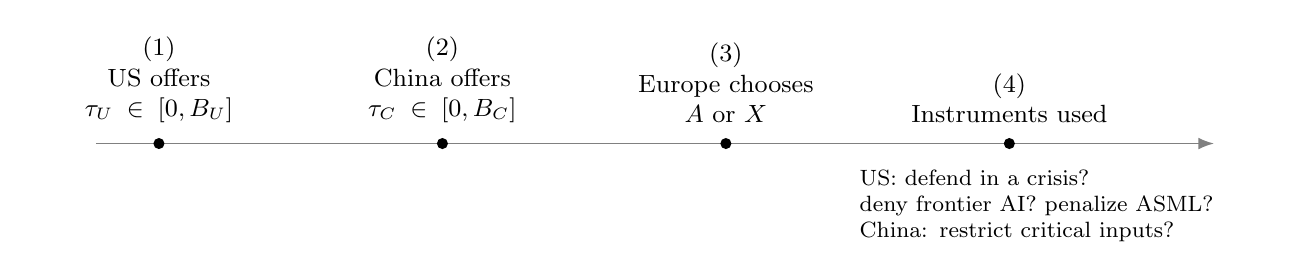
\begin{tikzpicture}[x=1cm,y=1cm,font=\small]
\draw[-{Latex[length=2mm]}, line width=0.6pt, gray] (0,0) -- (14.2,0);
\foreach \x/\lab/\who in {0.8/{US offers $\tau_U\in[0,B_U]$}/{(1)}, 4.4/{China offers $\tau_C\in[0,B_C]$}/{(2)}, 8.0/{Europe chooses $A$ or $X$}/{(3)}, 11.6/{Instruments used}/{(4)}}{
  \fill[black] (\x,0) circle (2pt);
  \node[above=4pt, align=center, text width=3.1cm] at (\x,0) {\who\\ \lab};
}
\node[below=6pt, align=left, text width=5.2cm, font=\footnotesize] at (12.3,0) {US: defend in a crisis?\\ deny frontier AI? penalize ASML?\\ China: restrict critical inputs?};
\end{tikzpicture}
\caption{Timing of the static game. Each instrument in stage (4) is used only if doing so is sequentially rational (\cref{lem:credible}).}
\label{fig:timing}
\end{figure}


\subsection{The price of alignment}\label{sec:bidding}

In the benchmark, Washington and Beijing bid for Europe's alignment in an ascending auction.

\begin{lemma}[Bidding benchmark]\label{lem:bidding}
Suppose the United States and China bid for Europe's alignment in an ascending (clock) auction in which bids are staked promises, Europe values China's promise $\tau_C$ at $\lambda_C\tau_C$, Europe chooses its alignment after the auction, and instruments are then used. Let $\bar z_U=\min\{V,\bar m_U\}$ and $Q=\lambda_C\min\{W_C,\bar m_C\}-c$.
\begin{enumerate}[label=(\roman*)]
\item After alignment $a$, the United States provides $x_j(a)$ for every instrument $j$, so exit lowers Europe's payoff, before transfers, by $c=\sum_j d_j+\eta$.
\item A promise of $\tau$ by power $i$ is honoured if and only if $\tau\le\bar m_i$. Bidding up to one's maximal credible bid (in units of Europe's payoff, $\bar z_U$ for the United States and $Q$ for China) is weakly dominant. In weakly undominated strategies, with an indifferent Europe aligning:
 \begin{enumerate}[label=(\alph*)]
 \item if $Q<V$ and $Q\le\bar m_U$, Europe aligns and the United States pays $\pos{Q}$;
 \item if $Q>\min\{V,\bar m_U\}$, Europe exits, and China's promise gives Europe $\min\{V,\bar m_U\}$ net of $c$.
 \end{enumerate}
 In both cases Europe's payoff is $\pos{\min\{Q,V,\bar m_U\}}$.
\item If $\bar m_U<Q<V$, every binding transfer $\tau\in[Q,V)$ from the United States to Europe would make both Europe and the United States strictly better off than the equilibrium (inefficient exit from limited US commitment).
\end{enumerate}
\end{lemma}

The losing bidder sets the price, a known result (\cref{sec:literature}) that \citet[Supplement B.2]{clayton2026framework} derive for two hegemons. What the lemma adds is the content of $Q$: China's bid enters Europe's participation constraint, and every cost of exit in $c$ is a conditional part that survives sequential rationality. In an alternating-raise auction, subgame perfection alone does not pin down the price if China is indifferent to what Washington pays (\cref{app:proofs}). A rival that values the patron's losses is not.

\begin{remark}[Price driving]\label{rem:spite}
In the alternating-raise auction, let China's relative-gains weight apply to every loss of Washington's, so that China gains $\rho p$ when Europe aligns at price $p$, with $\rho>0$. Let China bid up to its credibility bound $\bar b_C=\lambda_C\bar m_C-c\ge Q$, even where a winning bid would be unprofitable, and let $\bar b_C<\bar z_U-\varepsilon$. Then in every subgame-perfect equilibrium Europe aligns and the price is within $\varepsilon$ of $\pos{\bar b_C}$. If China's cap binds ($W_C\ge\bar m_C$), then $\bar b_C=Q$.
\end{remark}

China raises any bid that Washington will top, since it gains from what Washington pays and never has to honour a bid it does not win. The price is then pinned at China's credibility bound rather than at its willingness to pay. The two coincide when China's cap binds; otherwise what sets the price is how far Europe trusts China's promises, not what exit is worth to China.

\subsection{Agenda power and rupture risk}\label{sec:master}

We now give Europe a voice in the price. Europe and Washington bargain over a perpetual signed transfer flow $P$, with China's credible offer, and hence $Q$, open to Europe as an exit option throughout; $P<0$ means Europe concedes. Agreements bind while Europe's premium stays at $Q$.\footnote{They are enforced by the stake technology; we assume that Washington's cap covers the agreed transfer ($\bar m_U\ge V$ suffices) and that a European concession is a policy Europe would have to reverse publicly. If the premium moves, the two bargain again. A commitment by Europe that survives a change in its premium is what \cref{sec:control} prices.} Every $\Delta$ units of time, Europe proposes with probability $\beta\in[0,1)$ and Washington otherwise. After rejecting a US offer, Europe may exit, which yields flows $Q$ to Europe and $-V$ to Washington forever. If it does not, the dispute ruptures with probability $1-e^{-\lambda\Delta}$; otherwise the status quo continues with flows $(0,0)$, and both discount at rate $r\ge 0$. Rupture is realignment that neither government chooses, for instance after a change of government in The Hague or an unintended escalation: a threat that leaves something to chance \citep{schelling1960strategy}. A rupture puts the parties in the exit state until it is repaired, at rate $\phi\ge 0$, after which bargaining resumes; a chosen exit is permanent.

\begin{proposition}[Bargaining with an outside option and rupture risk]\label{prop:master}
Let $Q<V$, $\beta\in[0,1)$, $r,\lambda,\phi\ge 0$, $r+\lambda>0$, and $r>0$ if $\phi>0$.
\begin{enumerate}[label=(\roman*)]
\item For every $\Delta>0$, every subgame-perfect equilibrium gives Europe the same payoff $x^*(\Delta)$ and the United States $-x^*(\Delta)$.
\item If $\lambda>0$, the subgame-perfect equilibrium is unique (up to Europe's exit choice at one point of indifference, which does not affect payoffs), and agreement is immediate. If $\lambda=0$, there are also stationary equilibria with delay, with the same payoffs.
\item As $\Delta\to 0$, $x^*(\Delta)$ and the equilibrium offer and demand converge to
\begin{equation}\label{eq:master}
P^*=\max\big\{Q,\ \psi\big(Q+\beta(V-Q)\big)\big\},\qquad \psi=\frac{\lambda}{\lambda+r+\phi}\in[0,1].
\end{equation}
If $r+\phi>0$, the second term is the larger one if and only if $Q<\hat Q\equiv\lambda\beta V/(r+\phi+\lambda\beta)$.
\end{enumerate}
\end{proposition}

\begin{figure}[t]
\centering
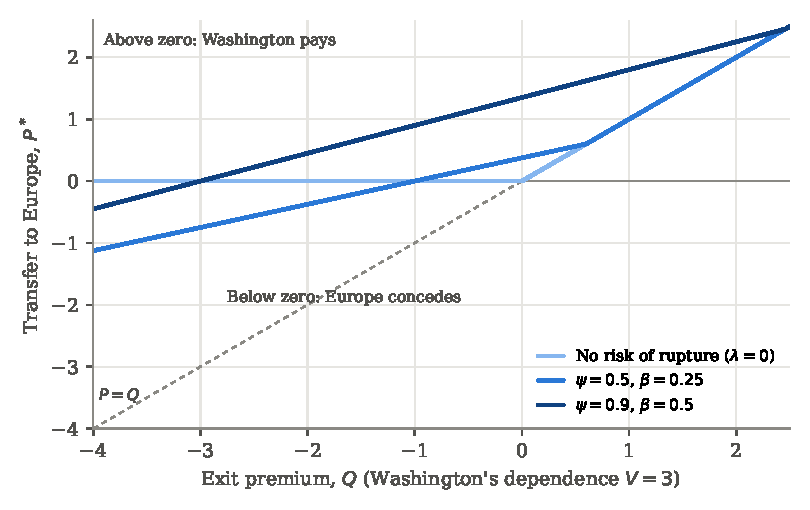
\includegraphics[width=0.75\textwidth]{figures/fig_master.pdf}
\caption{Equilibrium transfer to Europe under rupture risk (\cref{prop:master}) as a function of the exit premium, with $V=3$. Without rupture risk ($\lambda=0$) the transfer is $\pos{Q}$. With rupture weight $\psi=0.5$ and $\beta=0.25$, Washington pays Europe whenever $Q>-1$; with $\psi=0.9$ and $\beta=0.5$, whenever $Q>-3$. Below those values Europe concedes. Every curve lies on or above the dashed line $P=Q$.}
\label{fig:master}
\end{figure}

\begin{corollary}[Threshold and channels]\label{cor:master}
Under the conditions of \cref{prop:master}:
\begin{enumerate}[label=(\alph*)]
\item $P^*\ge Q$: Europe never concedes more than its slack, $-P^*\le\Lambda$.
\item If $\lambda=0$, $P^*=\pos{Q}$; if $\beta=0$, $P^*=\max\{Q,\psi Q\}$. In either case $Q\le 0$ implies $P^*\le 0$.
\item $P^*>0$ if and only if $Q>0$, or $\lambda>0$ and $Q+\beta(V-Q)>0$.
\item Holding $Q$ fixed, $\partial P^*/\partial V=\beta\psi$ where the second term binds ($Q<\hat Q$) and $0$ where $Q>\hat Q$.
\item $V$ enters $P^*$ directly only through the term $\beta\psi V$ (agenda power under rupture risk), and indirectly only through $Q$: through the rival's valuation ($\rho V$ in $W_C$ when the cap does not bind), self-harming sanctions ($\chi_f$ falls to zero as $V$ rises past $(\gamma+\bar m_U)/c_f$) and the silicon shield (if $s_B$ rises with $V$, $\kappa$ moves with a sign that depends on $G$). \Cref{prop:pain} adds a fifth channel, hold-up, which works through Washington's own need for ASML's servicing.
\end{enumerate}
\end{corollary}

The threshold in part (b) is the outside-option principle, and its substance is \citeauthor{wagner1988economic}'s (\cref{sec:literature}). Without rupture risk, a holder whose exit premium is negative gets nothing for its chokepoint, whoever proposes and however much its patron needs it: its only threat is exit, and exit is credible only when $Q>0$. When $\lambda>0$, a rejected demand risks a rupture that costs Washington $V$, so Europe's demands carry weight in proportion to $\beta\psi$, a binary instance of the identity-dependent externalities through which a seller extracts surplus from parties that do not buy \citep{jehiel1996how}. Repair changes only the weight: as $r\to 0$, $\psi$ tends to $\lambda/(\lambda+\phi)$, the long-run share of time that a relationship subject to these shocks spends broken. If ruptures are quickly undone, as when a new government in The Hague would realign and its successor return, Washington's dependence counts only in proportion to how long a rupture would last. The corner $\beta\to 1$, $\lambda\to\infty$, $\phi=0$, in which Europe obtains all of $V$, is the bargaining implied when the summary of \citet{juijn2026europe} calls ASML ``the only card Europe still holds'' (\cref{sec:intro}). It requires take-it-or-leave-it demands whose rejection ends in lasting realignment with near certainty, a commitment Europe has not shown it can make.

Hold-up is the other route by which Washington's need for ASML can raise Europe's price. If disagreement carries flow costs $c_E$ to Europe and $c_U$ to Washington, as when Europe interrupts the servicing of US-aligned fabs, Europe's price becomes $\max\{Q,\ \psi(Q+\beta(V-Q))+(1-\psi)(\beta c_U-(1-\beta)c_E)\}$ with constant costs and permanent rupture (\cref{prop:pain}). \Cref{sec:extensions} summarizes when such an interruption is credible.

Rupture risk cuts both ways. When $Q<0$ and $Q+\beta(V-Q)<0$, a rupture would leave Europe worse off than the aligned status quo, and Washington can extract part of the value to Europe of avoiding it, though never more than Europe's slack (\cref{cor:master}(a)). \Cref{sec:slack} shows that Europe's surplus over exit, whatever bargaining produces it, also caps what Washington obtains by any combination of conditional threats.

\section{The Slack Principle}\label{sec:slack}

\Cref{lem:bidding} and \cref{prop:master} price the chokepoint. On our reading of the record since 2019 (\cref{sec:evidence}), Europe's premium has been negative, and Washington has still asked Europe for a great deal. A patron can obtain the holder's surplus over exit, plus whatever it can threaten that does not depend on the holder's alignment. We state this for any rule that settles Europe's price at the end of a period, so that one result covers the bidding benchmark, bargaining under rupture risk, hold-up and price driving.

\subsection{Bite, budgets and assurance}\label{sec:slackprinciple}

Consider one period in which Europe is aligned and its premium is $Q$. Washington has finitely many demands. Demand $k$ costs Europe $t_k>0$ and is worth $w_k>0$ to the United States. A concession is \emph{reversible} if exit would undo it, so that it lowers Europe's aligned payoff and leaves its exit payoff unchanged. A concession is \emph{sunk} if it lowers both payoffs: payments, purchases, and transfers of assets or of control over them. \Cref{sec:linkage} shows that which concessions are reversible is itself a choice of Washington's.

\paragraph{Settlement.} At the end of the period Europe's price is settled at the premium then prevailing. Let $\mathcal P(q)$ be Europe's payoff from the settlement, relative to the aligned status quo, when its premium is $q$, and let $-\mathcal P(q)$ be Washington's. We require three properties: (S1) $\mathcal P(q)\ge q$, since Europe can always exit; (S2) $\mathcal P$ is nondecreasing; and (S3) $\mathcal P(q')-\mathcal P(q)\le q'-q$ for $q\le q'$, so that a higher premium never raises Europe's price by more than itself. Four settlements in this paper satisfy them while Washington retains Europe: the bidding payment $\mathcal P(q)=\pos{q}$ (\cref{lem:bidding}); bargaining under rupture risk, $\mathcal P(q)=\max\{q,\psi(q+\beta(V-q))\}$ (\cref{prop:master}), a maximum of affine functions with slopes $1$ and $\psi(1-\beta)$; hold-up with constant disagreement costs, which adds $(1-\psi)N$ to the second term (\cref{prop:pain}); and price driving, $\mathcal P(q)=\pos{q+\bar b_C-Q}$ (\cref{rem:spite}). Europe's \emph{surplus over exit} is $\Lambda_{\mathcal P}=\mathcal P(Q)-Q\ge 0$. In the bidding benchmark it is the slack $\Lambda=\pos{-Q}$.

\paragraph{Instruments.} Washington backs its demands with instruments (\cref{sec:security}). Withdrawing a set $J$ of instruments from an aligned Europe for the period lowers Europe's aligned payoff by $\Delta^A(J)$ and its exit payoff by $\Delta^X(J)$, with $0\le\Delta^X(J)\le\Delta^A(J)$ and both nondecreasing in $J$. We call
\[
u(J)=\Delta^X(J)\qquad\text{and}\qquad d(J)=\Delta^A(J)-\Delta^X(J)
\]
the unconditional and conditional parts of $J$. The conditional part is what Europe would lose by exiting anyway (for a single instrument, the $d_j$ of \cref{eq:Q}). The unconditional part is what Washington would still provide to an exited Europe and can threaten to take away. We impose no additivity: the AI instrument and US force posture may be complements or substitutes in Europe's payoff.

\paragraph{Ultimatums.} Washington's credible set $J^c$ is fixed at the start of the period, and no instrument outside it can be withdrawn. Washington issues \emph{adaptive ultimatums}: any sequence of demands, each naming unconceded demands and a threat set of instruments not yet withdrawn, each chosen after seeing Europe's earlier responses. If Europe refuses, Washington executes the threat at direct cost $e(J)\ge 0$, and executed instruments stay withdrawn for the period, so a threat once carried out is \emph{spent}. A threat that deters is not spent and can back the next demand. If $J_w$ has been withdrawn and Europe has made reversible concessions $T_{\mathrm r}$ and sunk ones $T_{\mathrm s}$, the settlement is played at the premium $Q+d(J_w)+T_{\mathrm r}$, and Europe receives $-\Delta^A(J_w)-T_{\mathrm r}-T_{\mathrm s}+\mathcal P(Q+d(J_w)+T_{\mathrm r})$. For a set $S$ of concessions, $T_{\mathrm r}(S)$ and $T_{\mathrm s}(S)$ are its reversible and sunk totals and $W(S)=\sum_{k\in S}w_k$ its value to Washington. Executing $J$ costs Washington $e(J)$ plus the rise in the settlement, which by (S3) is at most $d(J)$. After any history, executing a further set raises the premium by at most $\Delta^A(J^c)$, since $0\le d\le\Delta^A$. So if $e$ is nondecreasing, every subset of $J^c$ stays credible after every history when $\bar m_U\ge e(J^c)+\Delta^A(J^c)$, a condition the attainment claims below use and the bounds do not.

\begin{proposition}[Slack principle]\label{prop:slack}
Let the settlement $\mathcal P$ satisfy (S1)--(S3), let $\Lambda_{\mathcal P}=\mathcal P(Q)-Q$, and let
\[
B(J)=\Delta^A(J)-\big[\mathcal P\big(Q+d(J)\big)-\mathcal P(Q)\big],\qquad \varrho(T)=T-\big[\mathcal P(Q+T)-\mathcal P(Q)\big].
\]
No instrument outside $J^c$ can be withdrawn during the period, executing a withdrawal of $J$ costs the United States $e(J)\ge 0$ directly, and the United States retains Europe after every history.
\begin{enumerate}[label=(\alph*)]
\item \emph{Bite.} Refusing an ultimatum backed by $J$, issued when nothing has been conceded or withdrawn, costs Europe $B(J)$, net of the change in its settlement. $B$ is nondecreasing in $J$, and
\[ B(J)\le u(J)+\min\{d(J),\Lambda_{\mathcal P}\}, \]
with equality if the withdrawal holds Europe to its outside option ($\mathcal P(Q+d(J))=Q+d(J)$) or leaves its settlement unchanged ($\mathcal P(Q+d(J))=\mathcal P(Q)$). In the bidding benchmark equality always holds, $B(J)=u(J)+\min\{d(J),\Lambda\}$, and if $Q\ge 0$ only unconditional parts bite.
\item \emph{Reversible concessions.} Europe's net loss from reversible concessions totalling $T$ is $\varrho(T)\le\min\{T,\Lambda_{\mathcal P}\}$, with equality in the bidding benchmark. Faced with a single ultimatum that asks for reversible concessions $T_{\mathrm r}$ and sunk concessions $T_{\mathrm s}$ and is backed by $J$, Europe accepts if and only if $\varrho(T_{\mathrm r})+T_{\mathrm s}\le B(J)$.
\item \emph{One budget.}
  \begin{enumerate}[label=(\roman*)]
  \item In every subgame-perfect equilibrium of every adaptive sequence of ultimatums, Europe's total net loss is at most $B(J^c)$. Conditional instruments share one budget: $B(J)-u(J)\le\Lambda_{\mathcal P}$ for every $J$, and reversible concessions cost Europe at most $\Lambda_{\mathcal P}$ in total, however they are backed.
  \item The United States' equilibrium payoff is at most
  $V_1=\max\{W(S)-\mathcal P(Q+T_{\mathrm r}(S)):\ \varrho(T_{\mathrm r}(S))+T_{\mathrm s}(S)\le B(J^c)\}$, the payoff of the best single ultimatum backed by $J^c$.
  \item If every subset of $J^c$ stays credible and the United States can commit to a single ultimatum, one bundled ultimatum backed by $J^c$ yields $V_1$. Europe's loss then equals $B(J^c)$ if the United States has a divisible sunk demand of positive value and of size at least $B(J^c)$.
  \end{enumerate}
\item \emph{Assurance.} Without that commitment the United States still obtains $V_1$ if all demands are reversible and $B(J^c)\ge\Lambda_{\mathcal P}$, or if some best single ultimatum contains all of its demands. (In every equilibrium if $e(J)>0$ for every nonempty $J$, as with additive execution costs that are positive for each instrument; in some equilibrium otherwise.) In general it can obtain strictly less. Threats that deter are not spent, so the United States reuses them after Europe concedes, and Europe anticipates this. With one instrument with $d=0$ and $n$ identical sunk demands of cost $\tau$, the United States obtains exactly $n \bmod (b+1)$ of them, where $b=\lfloor B(J^c)/\tau\rfloor$.
\end{enumerate}
\end{proposition}

\Cref{app:proofs} has the proof and \cref{app:numerics} the brute-force checks. The proof uses only (S1)--(S3). Withdrawing a conditional part from an aligned Europe takes away something Europe would lose by exiting anyway, so it raises Europe's premium by $d(J)$. In the bidding benchmark the withdrawal hurts Europe up to $\Lambda$. Beyond $\Lambda$ the premium turns positive and Washington must pay rent to keep Europe aligned, which hands the excess back. A reversible concession works the same way, which is part (b): it lowers only the aligned payoff, so past $\Lambda$ Europe would exit unless compensated. Sunk concessions and unconditional parts escape the cap because they hurt Europe whatever it does.

The same holds whatever settles the price. Under rupture risk, agenda power can lift Europe's price above $\pos{Q}$, and the budget becomes $\Lambda_{\mathcal P}=P^*(Q)-Q$, which grows with $V$ while agenda power binds. It can also be smaller than $\Lambda$: when rupture risk makes Europe concede in the bargaining ($P^*(Q)<0$), threats can extract only the rest of its surplus over exit. Take $Q=-1$, $V=4$, $\beta=0.5$, $\lambda=1$, $r=0.25$ and $\phi=0$. Then $\Lambda=1$ and $\Lambda_{\mathcal P}=2.2$, and withdrawing a conditional part of $3$ costs Europe $1.8$. Whatever agenda power, hold-up or a rival's price driving wins Europe above its outside option, credible conditional threats can claw back, down to the exit premium. The agenda channel of \cref{cor:master}(e) therefore survives only to the extent that Washington lacks credible conditional threats large enough to push Europe to its outside option. Where the second term of $P^*$ binds, the settlement also rises at rate $\psi(1-\beta)$ with the premium, so a reversible concession of $T$ inside the budget costs Europe only $(1-\psi(1-\beta))T$: rupture risk returns part of every reversible concession.

\begin{figure}[t]
\centering
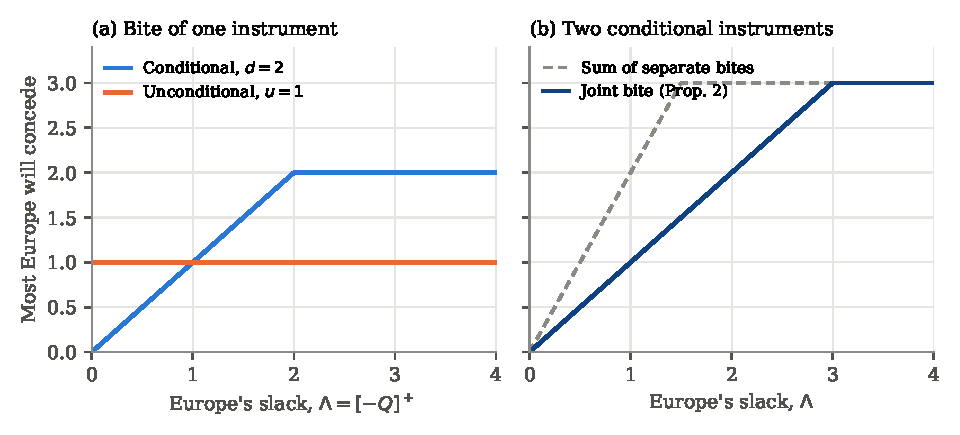
\includegraphics[width=0.95\textwidth]{figures/fig_slack.pdf}
\caption{The slack budget in the bidding benchmark. Panel (a): the bite of a conditional instrument with $d=2$ rises one for one with Europe's slack $\Lambda$ until $\Lambda=2$; an unconditional instrument with $u=1$ bites the same at every $\Lambda$. Panel (b): two conditional instruments with $d=1.5$ each. The sum of their separate bites (dashed) overstates their joint bite $\min\{3,\Lambda\}$ at every $\Lambda<3$. Bites from \cref{prop:slack}(a).}
\label{fig:slack}
\end{figure}

In panel (a) of \cref{fig:slack} the unconditional threat is the smaller one, yet it is the only one that still works as $\Lambda$ falls toward zero. Panel (b) illustrates part (c)(i). A coercer that prices each conditional threat on its own counts the same slack twice: at $\Lambda=1$ the separate bites sum to $2$ and the joint bite is $1$. The bound in (c)(i) needs only a fixed credible set (\cref{app:numerics}). Attaining it needs that set to stay credible after every history, which the cap condition stated before the proposition ensures.

Part (d) is the assurance problem of a coercer that cannot commit to stop demanding. Europe concedes only if everything the unspent threat will extract later stays within the bite. With $b+1$ identical sunk demands, a single ultimatum obtains $b$ of them. The adaptive sequence obtains none. A threat meant to induce compliance works only if the target believes compliance will end it \citep{schelling1966arms}, and \citet{pauly2024damned} shows that the steps that make a threat credible weaken that belief. A staked promise to make no further demand in the period buys the commitment. Stakes cost nothing. Part (d) therefore describes a patron whose cap $\bar m_U$ is small relative to the value of its later demands. Such a patron can gain by issuing an ultimatum it expects Europe to refuse, which burns an instrument that would otherwise back later demands (\cref{app:numerics}).

\begin{corollary}[Rationing]\label{cor:rationing}
In the bidding benchmark, suppose all demands are reversible and either the United States can commit to a single ultimatum or $B(J^c)\ge\Lambda$. Then its optimal demand set solves
\[ \max_{y_k\in\{0,1\}}\ \sum_k w_k y_k-\pos{\textstyle\sum_k t_k y_k-\Lambda}
   \quad\text{s.t.}\quad \min\Big\{\sum_k t_k y_k,\Lambda\Big\}\le B(J^c), \]
with one $y_k$ for each demand $k$. This is the knapsack $\max\sum_k w_k y_k$ s.t.\ $\sum_k t_k y_k\le\min\{\Lambda,B(J^c)\}$ if $B(J^c)<\Lambda$, or if demands are divisible ($y_k\in[0,1]$) and $w_k\le t_k$ for every $k$. In general the United States may exceed $\Lambda$ and pay the excess back as rent. The free capacity $\min\{\Lambda,B(J^c)\}$ falls as $Q$ rises toward $0$. Demands from every issue area draw on it.
\end{corollary}

With a general settlement the objective is $\sum_k w_ky_k-[\mathcal P(Q+\sum_kt_ky_k)-\mathcal P(Q)]$, and capacity is free only where $\mathcal P$ is flat.


\section{Linkage and Refusals}\label{sec:linkref}

The slack principle treats a concession's reversibility as given. This section makes it a choice of Washington's, which determines which demands compete for Europe's slack, and then asks why, in a model in which every demand is priced in advance, Europe ever refuses one.

\subsection{Which demands compete}\label{sec:linkage}

Whether a concession is reversible depends on what enforces it. In \cref{prop:slack} the only thing that holds Europe to a reversible concession is the threat of losing the conditional parts of Washington's instruments, so a Europe that exited would undo every such concession at once. That is why they share one budget. Washington can also enforce a concession with a penalty of its own, attached to the issue and not to Europe's alignment: a tariff threat behind a trade concession, or a sanction behind a purchase commitment.

Let demand $k$ carry an \emph{issue-specific penalty} $p_k\in[0,\infty]$: a staked threat, credible whatever Europe's alignment, to impose a loss $p_k$ on Europe if it reverses concession $k$. A payment that cannot be recovered has $p_k=\infty$. Washington \emph{links} a set $L$ of demands: it treats the reversal of a linked concession as exit, so reversing one while staying aligned gives Europe no more than exiting would. At the end of the period Europe chooses its alignment and which concessions to reverse.

\begin{proposition}[Linkage]\label{prop:linkage}
Maintain the assumptions of \cref{prop:slack}, with the penalties $p_k$ and the linked set $L$ as above.
\begin{enumerate}[label=(\alph*)]
\item \emph{Enforced and linked parts.} An aligned Europe delivers concession $k$ if and only if $k$ is linked or $t_k\le p_k$. Its \emph{enforced part} $\min\{t_k,p_k\}$ enters Europe's payoffs as a sunk concession, and its \emph{linked part} $\pos{t_k-p_k}$, when $k\in L$, as a reversible one. \Cref{prop:slack} holds with $T_{\mathrm s}(S)=\sum_{k\in S}\min\{t_k,p_k\}$ and $T_{\mathrm r}(S)=\sum_{k\in S\cap L}\pos{t_k-p_k}$.
\item \emph{Where demands crowd each other out.} Demands draw on the shared budget $\Lambda_{\mathcal P}$ only through their linked parts. If $t_k\le p_k$ for every demand, no demand needs linkage, accepted demands leave the settlement unchanged, and demands interact only through the bite constraint $\sum_{k\in S}t_k\le B(J^c)$. Linking a demand with $t_k\le p_k$ changes nothing.
\item \emph{Who gains from separate enforcement.} For a given set of concessions, raising $p_k$ weakly raises Europe's loss and weakly lowers the settlement Washington pays. If $B(J^c)\ge\sum_k t_k$, the payoff $V_1$ of Washington's best single ultimatum is nondecreasing in each $p_k$.
\end{enumerate}
\end{proposition}

The one budget of \cref{prop:slack} is thus the case in which Washington's only enforcement of reversible demands is the alliance itself ($p_k=0$). The more Washington can enforce a concession with a penalty that does not run through Europe's alignment, the less that concession draws on Europe's slack, and the more it costs Europe, because exit no longer undoes it. Europe's protection against an accumulation of demands is that they can be undone together. Crowding out through the slack should therefore appear between demands enforced only by linkage, and not between demands that Washington enforces separately, which interact only through the bite of its threats. That makes the cross-issue budget a claim about how Washington enforces its demands, which can be observed.

Export-control alignment and limits on servicing in China are enforced by linkage, beyond what flow jurisdiction blocks directly (\cref{sec:background}). The trade terms of August 2025, under which the EU said it would eliminate tariffs on US industrial goods and align its technology-security requirements with US ones \citep{whitehouse2025jointstatement}, are enforced at least partly by the threat of higher US tariffs, so only the part of them that a tariff threat cannot hold draws on Europe's slack. The NATO spending target for 2035 \citep{nato2025hague} and the EU's stated intention to buy more US military equipment \citep{whitehouse2025jointstatement} are closer to sunk, since they cost Europe whatever it later does with ASML. They draw on the bite of Washington's instruments and not on the slack. At The Hague in June 2025 Trump tied Spain's trade terms to its defence spending: ``We're negotiating with Spain on a trade deal. We're going to make them pay twice as much'' \citep{rte2025nato}. In our terms that is linkage, which Washington needs where an issue-specific penalty cannot hold a concession on its own.

China can tax a linked concession too. A Chinese counter-threat attached to a particular concession, announced before Washington moves, adds to that concession's cost exactly as a sunk cost would. If Washington has other demands China cannot reach, it fills the bite with them, so the counter-threat changes Washington's demand mix and taxes the patron rather than the holder, and China carries out a threat only to crowd out another demand (\cref{prop:counter} in \cref{app:counter}). \Cref{sec:record} reads the Nexperia episode against that requirement.

\subsection{Refusals}\label{sec:refusals}

Under complete information no demand is refused and no threat is carried out: Washington never makes a demand that Europe would resist. Yet Europe has resisted demands, such as limits on servicing in China (\cref{sec:intro}). A refusal needs Washington to be unsure what a demand would cost Europe. Let the net cost to Europe of one demand, $\kappa$, be Europe's private information, drawn from a continuous distribution $F$; its sign is unrestricted, since Europe may want some steps for its own reasons. To keep the settlement fixed, we let the demand be enforced ($t\le p$ in \cref{prop:linkage}), so that accepting it lowers Europe's aligned and exit payoffs equally. Washington values the concession at $w>0$, chooses a threat set $J\subseteq J^c$ before Europe responds, and carries out a refused threat. $J=\emptyset$ is an unbacked request, with $B(\emptyset)=0$. Executing $J$ costs Washington $E(J)=e(J)+\mathcal P(Q+d(J))-\mathcal P(Q)\ge 0$.

\begin{proposition}[Refusals and executed threats]\label{prop:refusal}
Under these assumptions Europe accepts if and only if $\kappa\le B(J)$, and the United States chooses $J$ to maximize $F(B(J))\,w-\big(1-F(B(J))\big)E(J)$.
\begin{enumerate}[label=(\alph*)]
\item In equilibrium the demand is refused with probability $1-F(B(J^*))$, and a refused demand that was backed ($J^*\neq\emptyset$) is followed by the execution of its threat. No threat set holds refusals below $1-F(B(J^c))\ge 1-F\big(u(J^c)+\min\{d(J^c),\Lambda_{\mathcal P}\}\big)$. With purely conditional instruments in the bidding benchmark this floor is at least $1-F(\Lambda)$, which rises as $Q$ rises toward $0$.
\item An unbacked request is refused with probability $1-F(0)$ and costs nothing when refused. Whenever $F(0)>0$, the United States prefers an unbacked request to no demand, so it always makes some demand, and if the demand it makes is unbacked, a refusal has no consequence.
\item Selecting the optimal threat set with the largest bite, $B(J^*)$ is nondecreasing in $w$: more valuable demands are backed by larger threats and are refused less often.
\item A refused and executed conditional threat raises Europe's premium by $d(J^*)$ and is spent for the rest of the period.
\end{enumerate}
\end{proposition}

The proposition says what the record should show. Near a zero premium, conditional threats bite little, so the refusals that Washington can prevent at any price become fewer (part (a)); the equilibrium refusal rate need not rise, since Washington may then switch to unconditional instruments or stop backing its demands. Requests that Washington does not back can be refused at no cost (part (b)). And the most valuable demands should come with the largest threats (part (c)). Dutch and Japanese resistance to limits on servicing in China fits an unbacked request better than a refused threat if, as the sources we use suggest, no US withdrawal followed it. The MATCH Act would back the request with a statutory deadline, but it had not been enacted by late October 2026 (\cref{sec:background}).


\section{Extensions}\label{sec:extensions}

The online supplement develops four extensions. Each takes the slack principle as given and asks what it implies for a question the core model leaves open.

\paragraph{Conditionality as a choice.} Washington chooses how conditional its guarantee is, through the stake $m_S$ on abandoning a realigned Europe in \cref{eq:kappa}. Conditionality lowers Europe's premium but costs Washington allied assurance. A patron with no demands beyond alignment makes its guarantee just conditional enough to hold the premium at zero; only a patron that plans to spend slack makes it more conditional, so conditionality is the price of concessions (\cref{prop:conditionality}). The cost need not be assumed. If a second ally values its own alignment less when it sees Europe's guarantee made conditional, conditionality toward Europe spends that ally's slack, and Washington stops where the spillover outweighs Europe's stake in the guarantee (\cref{rem:assurance}).

\paragraph{Preventive control.} The premium moves over time. A Washington that expects to pay Europe later, and cannot hold Europe to a promise to forgo that payment, has a motive to demand control of ASML's customers, output and technology while its threats still bite (\cref{prop:control}). Because the conditional part of the bite is capped by current slack, a coerced demand comes in windows while Europe is weak but expected to grow stronger (\cref{cor:windows}), and an autonomy investment that Europe cannot commit to forgo strengthens the motive (\cref{cor:control}). The motive needs a surplus that a transfer would remove, not a positive premium: under rupture risk it can arise while Europe's premium stays negative (\cref{rem:controlsettle}). Binding itself through EU-level controls protects Europe only if Washington values control little for its own sake (\cref{rem:bind}), and a credible Chinese threat to punish a transfer protects European ownership without being carried out (\cref{cor:control}(d)).

\paragraph{Who decides.} Exit toward China is a Dutch licensing decision, while turning ASML against Washington needs the Union, because its most advanced tools ship to US fabs under a Union general authorisation. A benefit aimed at The Hague alone buys alignment at a discount (\cref{rem:gatekeeper}); Chinese penalties for complying with US measures can make ASML ship where The Hague licenses it (\cref{rem:firm}); and Washington can defeat a countermeasure by buying a blocking minority before the Council's determination, though the record points to a cheaper route, a concession that triggers suspension (\cref{rem:council}, \cref{sec:council}).

\paragraph{Hold-up.} Europe could interrupt ASML's servicing of US-aligned fabs during a dispute. That raises Europe's price only for the servicing Washington cannot compel, and only if Washington's stock of spare parts and repair capacity runs out soon enough (\cref{cor:interrupt}). If Europe fixes its choice before offers in each round, every equilibrium gives the same answer. If it can lift an interruption after any US offer, as the Union's instruments allow, there are equilibria in which the threat to interrupt works at full strength without ever being used and equilibria in which it is worthless (\cref{prop:range}). On our reading the Union's record of suspending each countermeasure it armed against Washington fits the second.

\section{The Record as a Plausibility Probe}\label{sec:evidence}

The parameters of the model are not measured, and a negative exit premium can rationalize almost any act of compliance after the fact. Compliance also cannot separate coercion from shared threat perception, because successful coercion ends at the threat stage \citep{drezner2003hidden}. What follows is not a test (\cref{sec:tests}).

\subsection{Observable implications}\label{sec:predictions}

\Cref{tab:implications} sets seven implications beside four rival accounts. Under shared threat perception the Netherlands aligns because it shares Washington's security concerns, as the cabinet says it does ``in general terms'' \citep[our translation]{tk2026match}; in the model that is a large intrinsic cost of exit $\eta$. In \citet{lake2009hierarchy} compliance is owed under a social contract in which the patron provides order and protection. In \citet{morrow1991alliances} the protégé trades autonomy for security. Under cost minimization a coercer prices each demand, one at a time, at a fixed cost of the cheapest credible instrument.

\begin{table}[!tbp]
\centering
\scriptsize
\setlength{\tabcolsep}{3pt}
\caption{Observable implications of the model and of rival accounts}\label{tab:implications}
\begin{tabularx}{\textwidth}{@{}>{\raggedright\arraybackslash}p{2.35cm}*{5}{>{\raggedright\arraybackslash}X}@{}}
\toprule
Implication (result) & This model & Shared threat perception (large $\eta$) & Hierarchy & Autonomy--security trade-off & Cost minimization\\
\midrule
Threshold (\cref{cor:master}) & Holder is paid only if $Q>0$, or if talks risk rupture and it has agenda power & No payment; holder aligns for its own reasons & No payment; compliance is owed & Protection is the payment & No prediction about payment\\
\addlinespace
Linkage only with slack (\cref{prop:counter}(b)) & Linkage against a hedge worth less to the patron than to the holder appears with slack and fades as $Q\to0$; flow jurisdiction does not track $Q$ & Little coercion of any kind & Commands need no threats & Protection is linked to autonomy throughout & Cheapest instrument at fixed cost\\
\addlinespace
One budget across linked demands (\cref{prop:slack}(c), \cref{prop:linkage}) & Demands enforced only through the alliance are substitutes within a period, demands enforced by their own penalties are not; the budget shrinks as the rival's offer rises & Issue areas independent & Authority bounded issue by issue by the social contract & One autonomy price for security, set within the alliance & Instruments priced separately at fixed cost\\
\addlinespace
Refusals (\cref{prop:refusal}) & The refusals that threats can prevent shrink as $Q\to0$; unbacked requests refused without consequence & Few demands and few refusals & Refusal is insubordination and is punished & No prediction & Refusals where the instrument costs more than the demand is worth, unrelated to $Q$\\
\addlinespace
Counter-threats (\cref{prop:counter}(a)) & Change the patron's demand mix and tax the patron; executed only to crowd out other demands & Holder absorbs them and keeps aligning & Patron shields its subordinate from third parties & No prediction & No prediction\\
\addlinespace
Rival bids (\cref{prop:conditionality}(c)(i)) & A stronger bid elicits a more conditional guarantee and no payment, while assurance is cheap & No response needed & Patron must provide more order to keep its authority & Better terms for the protégé & No prediction\\
\addlinespace
Preventive control (\cref{prop:control}, \cref{cor:windows}) & Control, or binding, is demanded while the holder is weak but expected to strengthen & No demand & More control where dependence is deeper, with no window & No prediction & Control demanded whenever cheapest, with no window\\
\bottomrule
\end{tabularx}
\par\smallskip
\begin{minipage}{\textwidth}\scriptsize
\emph{Note.} Rival-account entries are our derivations from \citet{lake2009hierarchy}, \citet{morrow1991alliances} and the definition of a cost minimizer in the text, not claims their authors make about these cases. $Q$ is the exit premium (\cref{def:Q}).
\end{minipage}
\end{table}

The threshold separates the model from hierarchy and the autonomy--security trade-off only through holders with a positive premium, which should be paid, as Kyrgyzstan was for Manas (\cref{sec:literature}). The third row discriminates most. Under cost minimization the instruments used on one demand do not change the price of another, while in our model a concession on one linked demand leaves less to extract on another. A concession that Washington enforces with a penalty of its own, as when trade terms are backed by a tariff threat, does not (\cref{prop:linkage}), which makes the prediction easier to refute. The second row separates the two only if instrument costs are fixed, since a coercer that counts the rent of \cref{prop:counter}(b) as a cost of linkage predicts the same switch. \Cref{prop:slack}(d), in which an added demand can lower what a patron with small stakes obtains, also separates the model from any coercer that prices demands one at a time.

\subsection{Coding transfers and threats}\label{sec:coding}

Reading the record through \cref{prop:master} requires a line between a payment and a threat never carried out. We draw it at Washington's ex post optimal provision to an aligned ally, the baseline $x_j(A)$ of each instrument (\cref{sec:security}). A \emph{transfer} exceeds that baseline and enters $P^*$. A \emph{threat left unexercised} is a baseline benefit that Washington would withdraw after exit, or a sanction it could impose and does not. It enters the exit cost $c$ as a conditional part $d_j$, however valuable it is to the holder.

Because the baseline cannot be observed, we code a benefit as baseline provision when it is extended to allies that took no comparable step, justified by the recipient's own capacity or alliance status, and revocable by rule, and as a transfer when it is created in response to the holder's step, withheld from comparable allies and framed as compensation. Supplement No.~4 meets all three baseline criteria (\cref{sec:background}), so we code it as a threat left unexercised, equivalently a reward for self-binding (\cref{rem:bind}), and code the favourable treatment that the National Security Strategy offers aligning countries the same way (\cref{sec:conditionality}).

The instrument behind a US demand is \emph{flow jurisdiction} if it reaches China-bound flows directly (de minimis and foreign direct product rules, entity listings, licences for US-origin items), \emph{conditional linkage} if it threatens to withdraw something in another domain that an exited holder would lose anyway (posture, AI access, trade terms), and \emph{unconditional} if it hurts the holder whatever it does. Chinese responses are counter-threats if announced before the holder concedes and executed if carried out.

Leverage in the model is the transfer, but the model also reads delay, the scope of the holder's controls, retained jurisdiction (self-binding with the key kept in Europe, \cref{rem:bind}) and tolerated hedges. A tolerated hedge is rationing (\cref{cor:rationing}) if only linkage could stop it, and a flow threat not yet credible if Washington could not stake the cost of blocking the flow itself (\cref{prop:counter}(b)).

\subsection{The Dutch record and Nexperia}\label{sec:record}

\paragraph{Alignment without a price.} Since 2019 The Hague has aligned in steps, from 2023 each following a US move (\cref{sec:background}), and under our rules it received no transfer. By \cref{cor:master}(b), the record is consistent with a premium that has been negative throughout if talks carry no risk of rupture or Washington makes the offers. The absence of payment identifies less than it seems to. Because $V$ is large for ASML, rupture risk combined with Dutch agenda power would imply a positive transfer unless $Q\le-\beta V/(1-\beta)$ (\cref{cor:master}(c)), and since $P^*$ approaches $\pos{Q}$ continuously as $\lambda\to 0$, a small payment cannot be told apart from none. Reading the record as $Q\le0$ therefore assumes that The Hague could not make demands whose rejection risked realignment, that a realignment would soon be undone, so that the rupture weight $\psi=\lambda/(\lambda+r+\phi)$ is small (\cref{prop:master}), or that Washington's credible conditional threats took back what agenda power would have won (\cref{prop:slack}).

The negative premium needs no security term. US flow jurisdiction over China-bound tools makes $\theta$ large, which shrinks both what China gains from exit and the relative gain it values, so $\omega$ is small unless China's cap binds (\cref{eq:omega}). ASML's US entities and staff are US persons (\cref{sec:background}), so the firm would not ship against a credible US penalty even if The Hague licensed exit (\cref{rem:firm}). With $\kappa=0$ these terms alone can make $Q$ negative. We have found no Chinese offer conditioned on Dutch exit, and ASML's revenue in China is not one. The record is therefore consistent with a jurisdictional source of Europe's slack and leaves the security channel largely untested. We found no documented case that links US security commitments to ASML, although public documents cannot exclude private linkage: the January 2023 talks behind the Dutch and Japanese controls were led by the US national security adviser and also covered Ukraine \citep{durbin2023biden}.

\paragraph{Orders of magnitude.} The terms of \cref{eq:Q} can be bounded, not estimated, and we give orders of magnitude in euros a year. The conditional part of the AI instrument, $d_{ai}$, is Europe's loss from moving from aligned to exited access to US frontier AI. It runs from about EUR 4 billion if European gains from AI are limited by adoption, through 50 billion, to 130 billion if they are limited by frontier capability \citep{acemoglu2024simple, filippucci2025g7, epoch2026eci}. The conditional part of the core guarantee, $\kappa S_k$, is about 12.5 billion at $\kappa=0.10$ and a stake of 125 billion, a value between costings of replacing US protection that leave out nuclear deterrence \citep{iiss2025defending, burilkov2025defending}; for $\kappa$ between 0.02 and 0.30 it runs from 2.5 to 37.5 billion. China's counter-threat of halting inputs to Europe runs from about 3 billion, our assumption for graduated punishment, to 77 billion, the ECB's estimated loss from a sudden halt of critical-dependency imports from the China-led bloc, applied to EU output \citep{attinasi2025hidden}.

If Washington's AI threat is credible, then, the AI term is likelier than the core guarantee to decide the sign of $Q$. China's counter-threat is not a term in $Q$, since China has punished specific acts and not alignment (\cref{sec:security}); it bears on which concessions Washington can extract (\cref{prop:counter}) and on China's punishment $r^c$ of a transfer of control (\cref{cor:control}). China's offer $\omega$ has no good measure, and $d_{ai}$ and $\kappa$ are not independent in practice, since US protection has responded to allies' conduct on unrelated issues (\cref{sec:background}).

\paragraph{Slack spent and unspent.} The sales controls came in steps from 2023, while servicing in China continued at least into mid-2026 (\cref{sec:background}). If the sales controls were backed by flow jurisdiction, as \cref{tab:cases} codes them, they drew on no slack (\cref{prop:counter}(b)), and the late arrival of demands on servicing reflects the cost of the flow threat. Rationing would require that some Dutch sales steps of 2023--2025 were backed by conditional linkage, which we have not found; the general linkage of AI exports and favourable treatment to export-control alignment came in August and December 2025 (\cref{sec:counter}) and names no Dutch step. Until 2026 Washington had no credible jurisdictional block on servicing done by ASML staff in China, who are not, we think, US persons, and since China's 2021 blocking rules and Decrees 834 and 835, stopping it carries a Chinese counter-threat (\cref{sec:background}). Nor does timing separate coercion from shared threat perception: a like-minded holder that would lose sales to Japanese rivals by moving alone would also wait for US rules that bind them, a coordination problem that \citet{farrell2019weaponized} identify when hubs lie in several jurisdictions.

\paragraph{Nexperia.} The Nexperia dispute of 2025 is the one episode in which China executed a counter-threat against a Dutch step taken under US pressure. The Dutch minutes of a meeting with the State Department on 12 June 2025 concluded that it was ``almost certain the CEO will have to be replaced to qualify for the exemption from the entity list'' \citep[paras.~2.19--2.20; our translation]{gerechtshof2025nexperia}, a Dutch record of US views, not a formal condition. On 30 September, the day after the Affiliates Rule took effect \citep{bis2025affiliatesrule}, the economy minister took control of Nexperia under the Goods Availability Act, and the Enterprise Chamber suspended its chief executive in early October \citep{kst32637720, gerechtshof2025nexperia}. On 4 October China announced an export control aimed at Nexperia's Chinese plants \citep{kst32637720}. At Busan on 30 October Washington agreed to suspend the Affiliates Rule for a year from 10 November, and China to ``take appropriate measures to ensure the resumption of trade from Nexperia's facilities in China'' \citep{fmprc2025busan, whitehouse2025busan, bis2025affiliates}. On 19 November the minister suspended his order, citing Chinese export licences for Nexperia chips. The Enterprise Chamber's separate measures stayed in force \citep{kst32637_717}.

We read the episode as a US-backed demand met by an executed Chinese counter-threat. Under complete information, \cref{prop:counter}(a)(iii) allows execution on the path only when it crowds out another demand, which requires a Chinese threat known in The Hague and Washington before 30 September, a US demand that Washington shelved because the Nexperia concession had become expensive, and a Dutch government that conceded expecting to bear the cost. The alternative, outside the model, is that The Hague, and perhaps Washington, misjudged China's resolve. The public record establishes neither reading, and the reversal does not discriminate, since by then the rule behind the US demand had been suspended.

Europe bore the cost and was not compensated. By \cref{prop:counter}(a)(v) the counter-threat taxes the patron and not the holder only if Washington has a divisible sunk demand that China cannot reach, and the relief came through a US concession to China at Busan, which we do not read as a transfer to Europe. \Cref{sec:firm} takes up what the episode would imply for the cost of compelling a firm.

\paragraph{Servicing and MATCH.} A statute is a stake. The MATCH Act would make a flow threat against servicing credible if $e_F\le\bar m_U$, and such a threat leaves $Q$ unchanged and need not be carried out (\cref{prop:counter}(b)). Congress has not posted the stake: the bill has not moved since committee approval in April 2026 \citep{hr8170}. The Dutch answer was voice (\cref{sec:background}), which is consistent both with jurisdiction alone keeping the premium negative and with perceived conditionality having risen after the targeted US moves of 2026. With $Q<0$, voice and the hold-up of \cref{sec:holdup} are all a holder has.

\subsection{Comparison cases}\label{sec:cases}

\Cref{app:cases} codes four contemporary and three historical cases with the rules of \cref{sec:coding} (\cref{tab:cases,tab:history}). We found no holder paid in cash for aligning on a chokepoint. The currency is status that BIS grants and withdraws by rule (Supplement No.~4, validated end-user status, annual licences), which we code as exit costs. Every holder in scope has, we think, a nonpositive premium, so the cases cannot test the threshold of \cref{cor:master}. Resistance clusters on the installed base and on signed deals (servicing of Chinese fabs, Bonn's contract with Brazil). In the model these concessions cost the holder much relative to the remaining bite, though a cost minimizer facing expensive enforcement would also tolerate them.

\paragraph{Where the comparison strains the model.} A complete-information patron does not both collect and cut, yet Washington collected West German offsets and in 1967 agreed to redeploy up to 35,000 personnel \citep{frus1995foreignecon, frus1999germany, frus1995westerneurope}. The cut is unexplained unless keeping the troops was a transfer priced by the offsets, and FRUS does not let us tell whether it was. In 1957 twelve of sixteen CoCom members backed abolishing the China differential \citep{frus1989economicdefense, mastanduno1992economic}, a collective exit our single-holder model does not represent. In the Brazil case conditionality existed only in Bonn's beliefs \citep{frus2014westerneurope}.

\subsection{Designs that could test the model}\label{sec:tests}

\paragraph{An event dataset.} The unit would be a US demand on a holder of a chipmaking-equipment chokepoint (the Netherlands, Japan, South Korea, Germany) from 2019 to 2026, coded from gazettes, parliamentary records and filings for the instrument threatened (\cref{sec:coding}), the response, any compensation and any Chinese response. It should be built around the cross-issue budget. A concession in one issue area should lower what Washington extracts in another within the same period if both are enforced only through the alliance, and not if Washington enforces one of them with a penalty of its own (\cref{prop:slack}(c), \cref{prop:linkage}). Where the premium is near zero, Washington's threats should prevent fewer refusals, and requests that Washington does not back should be refused without consequence (\cref{prop:refusal}). Linkage against hedges should fade as the premium rises toward zero, while flow jurisdiction does not track it (\cref{prop:counter}(b)).

\paragraph{An elite survey experiment.} Conditionality is a property of US behaviour, so the respondents should be US foreign-policy elites. Vignettes would vary whether an ally holding a chokepoint complied with US controls, refused, or complied on sales while servicing Chinese fabs. The gap in support for defending the ally and keeping forces there estimates $\kappa$ and $d_p$. Further arms would vary a public presidential stake and whether Washington uses bases there (\cref{prop:conditionality}).

\paragraph{Process tracing.} Requests under the Dutch Open Government Act (Woo) for records of export-control talks with US counterparts since 2019 would show whether security commitments, posture or the F-35 programme were raised. They would also date Dutch drafting against US demands, which separates coercion from shared threat perception, and show what The Hague expected from China before 30 September 2025.

\paragraph{The Busan expiry.} If the suspensions agreed at Busan lapse (\cref{sec:background}), the rule behind the Nexperia demand and China's extraterritorial rare-earth controls return together \citep{bis2025affiliates, mofcom2025pause}. \Cref{prop:counter}(a) then leads us to expect Washington to shift its demands on The Hague toward demands China cannot reach or flow jurisdiction it exercises itself. A second executed counter-threat against a Dutch step would be hard to square with misjudgment, which learning should correct.

\section{Implications and Conclusion}\label{sec:conclusion}

\subsection{Scope}\label{sec:scope}

Four conditions define the class of cases: (i) \emph{security dependence}, protection the holder cannot replace on the relevant horizon ($S_k>0$); (ii) \emph{a partly conditional guarantee}, some of which the patron can stake to withhold after exit ($\kappa S_k+d_p>0$; \cref{prop:conditionality}); (iii) \emph{a rival that bids} ($\omega>0$); and (iv) \emph{a nested chokepoint}, partly inside the patron's jurisdiction while the holder's licence still decides exit ($0<\theta<1$). The Netherlands, Japan and South Korea meet the first and fourth. On the second, the May 2026 posture order against Germany (\cref{sec:background}) suggests that $d_p$ is positive; the conditionality of the core guarantee is largely untested (\cref{sec:record}). The third holds only weakly: we found no Chinese offer for any holder's exit, one reason we think $\omega$ is small. Taiwan (threatened by China, not courted) and the Gulf partners (no treaty guarantee) fall outside.

\subsection{Implications for Europe}\label{sec:implications}

We place Europe at a nonpositive premium with little rupture risk: The Hague has received revocable statuses, which we do not code as transfers (\cref{sec:coding}), and has made no demand whose rejection risked realignment (\cref{sec:record}). Washington's conditional threats can claim no more than Europe's slack (\cref{prop:slack}), so Europe gains by shrinking it.

\paragraph{Reduce the conditional part of dependence.} Against the NATO target of 5 percent of GDP by 2035 \citep{nato2025hague}, the model counts a euro only insofar as it replaces something Washington could withhold after exit: substitutes for posture and enablers more than duplicates of the statutory core (\cref{sec:security}), and AI capacity Washington cannot withhold, which lowers $d_{ai}$. While $Q<0$ a gain in premium removes slack one for one and brings no transfer (\cref{cor:rationing}). Where assurance is cheap at the margin, Washington answers with a more conditional guarantee and pays nothing (\cref{prop:conditionality}(c)(i)).

\paragraph{Keep concessions reversible together.} Because exit would undo Europe's reversible concessions at once, they share one budget, which protects Europe against an accumulation of demands. A concession that Washington can enforce with a penalty of its own, such as a snapback tariff, escapes that budget and costs Europe more (\cref{prop:linkage}). Europe gains from resisting issue-specific enforcement clauses even for concessions it accepts.

\paragraph{Shrink the jurisdictional source of slack.} Washington reaches ASML through US-origin inputs and US persons (\cref{sec:background}); on our reading that shared jurisdiction alone can keep the premium negative. Moving that content and servicing out of US jurisdiction lowers $\theta$, which raises $\omega$ only while China's cap does not bind (\cref{eq:omega}); the surer gain is a lower share $h$ of servicing that Washington can compel (\cref{sec:holdup}). In May 2026 The Hague opposed the MATCH Act's extraterritorial reach, arguing that ``every country is responsible for its own export control legislation'' \citep[our translation]{tk2026match}, which we read as a defence of who holds the key.

\paragraph{Interrupt servicing only under a rule that cannot be suspended.} Under the Union's timing, interruption helps only if both sides expect a rejected demand to be met by one (\cref{prop:range}), and each countermeasure the Union armed against Washington was suspended once Washington moved (\cref{sec:council,sec:holdup}). A credible option would need a legal basis, adopted before any dispute, that no EU body could suspend on a US offer, and Germany, whose Zeiss optics and Trumpf lasers cannot be commandeered abroad (\cref{sec:holdup}).

\paragraph{Expect a preventive demand; bind with care.} Washington demands control when the premium is negative but expected to turn positive and its credible bite is large enough (\cref{cor:control}(a), \cref{cor:windows}), and autonomy investments Europe cannot commit to forgo strengthen the motive (\cref{cor:control}(b)). Keeping the key in Europe, or binding as Delegated Regulation 2025/2003 \citep{eu2025dualuse} did partway (\cref{sec:bind}), deters a demand for control only if Washington values control little for its own sake (\cref{rem:bind}). US demands shifting toward ownership or a licensing veto would indicate a high $v_c$, under which binding raises the bite and pre-empts nothing.

\paragraph{Chinese counter-threats.} If Washington has a divisible sunk demand China cannot reach, as we read the spending target and purchases of US equipment (\cref{sec:slackprinciple}), de-risking, the aim of the Critical Raw Materials Act \citep{eu2024crma}, leaves Europe's loss at $B(J^c)$ (\cref{prop:counter}(a)). De-risking then pays mainly where China retaliates against Europe's own acts, as in Nexperia (\cref{sec:record}).

\subsection{Limitations}\label{sec:limits}

Complete information about conditionality is the strongest remaining assumption. \Cref{prop:refusal} lets Washington be unsure what a demand costs Europe, which produces refusals and executed threats. If $\kappa$ were private, Washington would gain from overstating it, and the 2025 National Security Strategy would be partly cheap talk. Refusals and executed counter-threats could then come from misjudgment, the reading of Nexperia outside the model (\cref{sec:record}), and conditionality could exist only in the holder's beliefs, as Bonn's fears in 1975--77 suggest (\cref{sec:cases}). The great powers are unitary, although Congress can set stakes the executive would not, as the MATCH Act's 150-day deadline would (\cref{sec:background}). With one rival and holders bargaining alone, the model is silent on whether a coalition of the Netherlands, Japan and South Korea would help.

\subsection{A third condition}

The floor and the slack principle add a condition to the theory of weaponized interdependence. \citet{farrell2019weaponized} require jurisdiction over a hub and the domestic institutions to use it. When a hub's holder bargains with a state that depends on it, a third condition applies: the holder's exit premium must be positive, unless it has agenda power under rupture risk (\cref{cor:master}(c)) or can impose hold-up (\cref{prop:pain}). The Netherlands licenses ASML's exports to China, so it has the institutions in that direction; turning the tools against Washington takes a Union decision (\cref{sec:council}). Both substitutes for a positive premium look weak to us, so whether it meets the third condition turns on China's credible promises and, if Washington's threat to withhold frontier AI is credible, on the AI instrument, which on our orders of magnitude weighs more than the conditional part of the guarantee (\cref{sec:record}).


{\raggedright
\bibliographystyle{aer}
\bibliography{refs}
}
\end{document}
